\documentclass{beamer}
\usepackage{inputenc}
\usepackage{tikz}
\usepackage{graphicx}
\usepackage{amsmath}
\usetheme{Berlin}
\usecolortheme{default}
\title{Assignment}
\subtitle{CS 213, Software Systems Lab}
\author[]{Ayush Mallick\\Computer Science and Engineering\\\href{mailto:220010008@iitdh.ac.in}{220010008@iitdh.ac.in}}
\institute[CSE, IIT Dharwad]{Indian Institute of Technology, Dharwad}
\logo{
\includegraphics[width=1cm]{logo.png}}
\begin{document}
\begin{frame}[plain]
\titlepage
\end{frame}
\begin{frame}[label=first]
Hello, this is our first frame. Here you can find info about IIT
Dharwad at the below mentioned link. \url{www.iitdh.ac.in} or by
clicking the following \href{www.iitdh.ac.in}{IIT Dharwad} name.
You can find info about super heroes by clicking at the following
button

You can find info about super heroes by clicking at the following
button. \hyperlink{superhero}{\beamergotobutton{Super Heroes}}

You can find info about mathematicians by clicking the following
button. \hyperlink{mathematicians}{\beamergotobutton{Mathematicians}}
\end{frame}

\section{Structures}

\begin{frame}
\frametitle{Structures}
    \only<1>{
    \begin{block}{Theorem: Magic}
        My name is Alt Temporal. I can do magic by changing myself in different slides.
    \end{block}{}
    \begin{alertblock}{The Truth}
        No don’t trust him he doesn’t do magic.
    \end{alertblock}
        }
    \only<2>{
    \begin{block}{Theorem: Magic}
        I have done the magic. You should have trusted me earlier before I have done the magic.
    \end{block}{}
    \begin{alertblock}{The Truth}
        I was just joking, The above person actually does the magic and also I can do it.
    \end{alertblock}{}
    }
\end{frame}


\begin{frame}
\frametitle{Structures with columns}
\setbeamercovered{transparent}
\begin{columns}
    \begin{column}{0.40\textwidth}
        \begin{alertblock}{Alert Column}
            Remain alert for the red light.
        \end{alertblock}
        \pause
        \begin{block}{ Test your Skills}
            There won't be any blue light at the signal
        \end{block}
        \pause
    \end{column}
    \begin{column}{0.40\textwidth}
        \begin{exampleblock}{To Go}
            Green light means to go past.
        \end{exampleblock}{}
        \pause
        \begin{exampleblock}{Extra Info}
            Green is also the color of this example block.
        \end{exampleblock}{}
            
    \end{column}
\end{columns}
     
\end{frame}

\section{Tables}
\begin{frame}
\frametitle{Table Frame 1}
\setbeamercovered{transparent}
\begin{table}[]
    \centering
    \begin{tabular}{ccc}
        \hline
        Our Sir in Google Meet & Student A & \\
        \pause
        & Student B & \pause \\ \hline
        Student C & Student D & Student E \\ \hline
    \end{tabular}
    \caption{Google Meet Interface as a Table with Teacher}
\end{table}

The table number shows teacher interacting with students in
Google Meet interface.
\end{frame}

\begin{frame}
\frametitle{Table Frame 2}
\begin{table}[]
    \centering
    \begin{tabular}{cc}
      \hline
      \multicolumn{2}{c}{Students}\\
      A & B\\
      \hline
    \end{tabular}
    \caption{Google Meet Interface without Teacher}
\end{table}

The table number shows students in Google Meet interface

\end{frame}

\begin{frame}
\frametitle{Table Frame 3}
\begin{table}[]
\setbeamercovered{transparent}
    \centering
    \caption{My Sample Table}
    \begin{tabular}{c|c|c|c}
        \textbf{Value 1} & \textbf{Value 2} & \textbf{Value 3} & \textbf{Value 4}\\
        \hline
        1 & 5 & 6 & 8 \\
        \pause
        2 & 9 & 11 & 13 \\
        \pause
        3 & 58 & 23 & 62
        \pause
    \end{tabular}
\end{table}

This is a sample table consisting of random things
    
\end{frame}

\begin{frame}
\frametitle{Table Frame 4}
\setbeamercovered{transparent}
\begin{table}
    \centering
    \caption{Students and their Marks}
    \begin{tabular}{ccccc}
        \uncover<1->{Sub} & \uncover<1->{A} & \uncover<2->{B} & \uncover<3->{C} & \uncover<4->{D} \\
        \uncover<1->{Mat} & \uncover<1->{35} & \uncover<2->{62} & \uncover<3->{93} & \uncover<4->{24} \\
        \uncover<1->{Phy} & \uncover<1->{32} & \uncover<2->{41} & \uncover<3->{56} & \uncover<4->{96} \\
        \uncover<1->{Che} & \uncover<1->{55} & \uncover<2->{83} & \uncover<3->{58} & \uncover<4->{92}
    \end{tabular}
\end{table}
\end{frame}

\section{Transitions}
\begin{frame}
\frametitle{Transition 1}
\transdissolve
Lorem ipsum dolor sit amet, consectetuer adipiscing elit. Ut purus
elit, vestibulum ut, placerat ac, adipiscing vitae, felis. Curabitur
dictum gravida mauris. Nam arcu libero, nonummy eget,
consectetuer id, vulputate a, magna. Donec vehicula augue eu
neque. Pellentesque habitant morbi tristique senectus et netus et
malesuada fames ac turpis egestas. Mauris ut leo. Cras viverra
metus rhoncus sem. Nulla et lectus vestibulum urna fringilla
ultrices. Phasellus eu tellus sit amet tortor gravida placerat.
Integer sapien est, iaculis in, pretium quis, viverra ac, nunc.
Praesent eget sem vel leo ultrices bibendum. Aenean faucibus.
Morbi dolor nulla, malesuada eu, pulvinar at, mollis ac, nulla.
Curabitur auctor semper nulla. Donec varius orci eget risus. Duis
nibh mi, congue eu, accumsan eleifend, sagittis quis, diam. Duis
eget orci sit amet orci dignissim rutrum.   
\end{frame}

\begin{frame}
\frametitle{Transition 2}
\transblindshorizontal
    Nam dui ligula, fringilla a, euismod sodales, sollicitudin vel, wisi.
Morbi auctor lorem non justo. Nam lacus libero, pretium at,
lobortis vitae, ultricies et, tellus. Donec aliquet, tortor sed
accumsan bibendum, erat ligula aliquet magna, vitae ornare odio
metus a mi. Morbi ac orci et nisl hendrerit mollis. Suspendisse ut
massa. Cras nec ante. Pellentesque a nulla. Cum sociis natoque
penatibus et magnis dis parturient montes, nascetur ridiculus mus.
Aliquam tincidunt urna. Nulla ullamcorper vestibulum turpis.
Pellentesque cursus luctus mauris.
\end{frame}

\begin{frame}
\frametitle{Transition 3}
\transblindsvertical
Nulla malesuada porttitor diam. Donec felis erat, congue non,
volutpat at, tincidunt tristique, libero. Vivamus viverra fermentum
felis. Donec nonummy pellentesque ante. Phasellus adipiscing
semper elit. Proin fermentum massa ac quam. Sed diam turpis,
molestie vitae, placerat a, molestie nec, leo. Maecenas lacinia.
Nam ipsum ligula, eleifend at, accumsan nec, suscipit a, ipsum.
Morbi blandit ligula feugiat magna. Nunc eleifend consequat
lorem. Sed lacinia nulla vitae enim. Pellentesque tincidunt purus
vel magna. Integer non enim. Praesent euismod nunc eu purus.
Donec bibendum quam in tellus. Nullam cursus pulvinar lectus.
Donec et mi. Nam vulputate metus eu enim. Vestibulum
pellentesque felis eu massa.
    
\end{frame}

\begin{frame}
\frametitle{Transition 4}
\transboxin
Quisque ullamcorper placerat ipsum. Cras nibh. Morbi vel justo
vitae lacus tincidunt ultrices. Lorem ipsum dolor sit amet,
consectetuer adipiscing elit. In hac habitasse platea dictumst.
Integer tempus convallis augue. Etiam facilisis. Nunc elementum
fermentum wisi. Aenean placerat. Ut imperdiet, enim sed gravida
sollicitudin, felis odio placerat quam, ac pulvinar elit purus eget
enim. Nunc vitae tortor. Proin tempus nibh sit amet nisl. Vivamus
quis tortor vitae risus porta vehicula.

\end{frame}

\section{Figures}
\begin{frame}
\frametitle{Great Mathematicians}
This frame shows pictures of Great Mathematicians
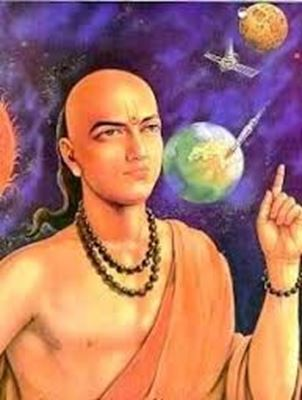
\includegraphics[height=5cm]{aryabhatta.jpeg}
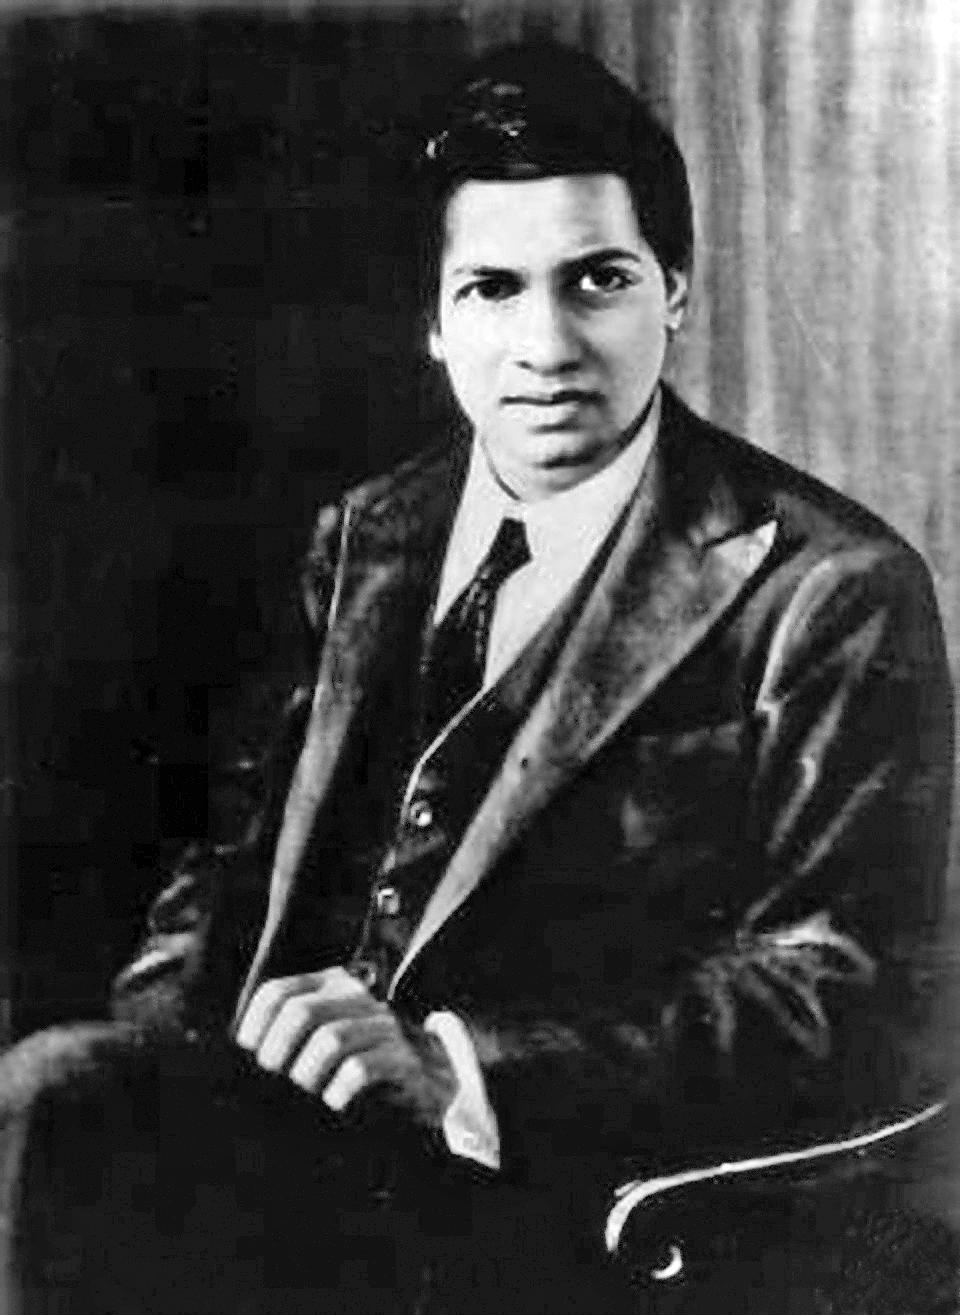
\includegraphics[height=5cm]{Srinivasa.jpg}
\end{frame}

\section{Mathematics}
\begin{frame}
\frametitle{Mathematics}
\setbeamercovered{transparent}
\uncover<1->{
Mathematics is a subject that we learn in the class. This is what
you may have known. But it’s something else. It’s a world of
numbers.}

\uncover<2->{
Mathematics consists of

1)Theorem or Proofs
}

\uncover<3->{
2)Equations

This is the last slide in Mathematics Intro
}

\end{frame}

\begin{frame}
\frametitle{Theorem or Proofs 1}

\begin{block}{Theorem: The Most Complicated One}
        $(a+b)^2 = a^2 + b^2 + 2ab$
\end{block}

\begin{exampleblock}{Proof:}
\begin{equation*}
       \begin{split}
           (a+b)^2 & = (a+b)(a+b) \\
           & = a^2 + ab + ba + b^2 \\
           & = a^2 + b^2 + 2ab
       \end{split}
\end{equation*}
\end{exampleblock}

\end{frame}

\begin{frame}
\frametitle{Theorem or Proofs 2}

\begin{block}{Theorem: The Second Most Complicated One}
        $(a-b)^2 = a^2 + b^2 - 2ab$
\end{block}

\begin{exampleblock}{Proof:}
\begin{equation*}
       \begin{split}
           (a-b)^2 & = (a-b)(a-b) \\
           & = a^2 - ab - ba + b^2 \\
           & = a^2 + b^2 - 2ab
       \end{split}
\end{equation*}
\end{exampleblock}
    
\end{frame}

\begin{frame}
\frametitle{Theorem Other Way}

\begin{theorem}
    Multiplication is not Commutative in Matrices.
\end{theorem}

\begin{proof}
    Ab is not equal to BA.
\end{proof}

\end{frame}

\begin{frame}
\frametitle{Equation -1}
\setbeamercovered{transparent}

This frame will consist of a multiline equation as follows:

Our Multiline Equation:

Area of Circle

\begin{equation}
    \begin{split}
        A & = \pi r^2 \\ \pause
        & = \frac{\pi d^2}{4}
    \end{split}
\end{equation}
    
\end{frame}

\begin{frame}
\frametitle{Equation -2}
\setbeamercovered{transparent}

\uncover<1->{
This frame will consist of onemore multiline equation as follows:

Our Multiline Equation:

Einstein's Equation:
}

\begin{equation*}
    \begin{split}
        E & = mc^2 \\ 
        \only<2>{
        & = (\sqrt{m}c)^2
        }
    \end{split}
\end{equation*}

\uncover<1>{
See magic converts single line eqn to multi line eqn}

\only<2>{
See I said no, I know magic, you should agree}
    
\end{frame}

\section{Our Section of Lists}

\begin{frame}
\frametitle{Our First List using itemize}
\setbeamercovered{transparent}

Hello
\begin{itemize}
    \pause
    \item This is first list item
    \item<2> This is second list item
    \item Thus is the final item which will be visible in all slides of the frame
\end{itemize}
    
\end{frame}

\begin{frame}[label=mathematicians]
\frametitle{Our Second List using enumerate}
\setbeamercovered{transparent}

Well known famous People
\begin{enumerate}
    \item \href{https://en.wikipedia.org/wiki/Aryabhata}{Aryabhatta}
    \pause
    \item \href{https://en.wikipedia.org/wiki/Albert_Einstein}{Einstein}
    \pause
    \item \href{https://en.wikipedia.org/wiki/Newton}{Newton}
    \pause
    \item \href{https://en.wikipedia.org/wiki/Niels_Bohr}{Bohr}\\
    You can find more info about them by clicking on their names or by searching at \href{www.google.com}{Google}
\end{enumerate}
    
\end{frame}

\begin{frame}[label=superhero]
\frametitle{Our Third List using Description}
\setbeamercovered{transparent}
\transdissolve

\begin{description}
    \uncover<2->{
    \item[Iron Man] His speciality is he wears a iron man suit.}
    \uncover<3->{
    \item[Thor] He has a hammer.}
    \item[Vivek] He know's how to use Beamer. 
\end{description}
\alert<3>{
Hereby all our lists are also completed}
 
\end{frame}

\begin{frame}{Our Final Frame that has Different Slides}
\only<1>{\textcolor{blue}{This frame is dedicated to the Beamer and people of IIT Dharwad
who are using it.}\\
\textcolor{red}{This is our final frame, and it says that all the given tasks are
completed by:}\\
\textcolor{blue}{To go back to the first frame after title click the following button.}
\hyperlink{first}{\beamerreturnbutton{Our First Frame}}
}
\only<2>{
\textcolor{blue}{This frame is dedicated to the Beamer and people of IIT Dharwad
who are using it.}\\
\textcolor{red}{This is our final frame, and it says that all the given tasks are
completed by:}\\
\textcolor{blue}{To go back to the first frame after title click the following button.}
\hyperlink{first}{\beamerreturnbutton{Our First Frame}}  

}
\end{frame}

\end{document}